\chapter{Abordagem da Engenharia de Requisitos}

  Scaled Agile Framework, ou SAFe, é utilizado para dimensionar processos ágeis para grandes projetos. Uma das filosofias do processo
  ágil é uma equipe pequena auto gerenciavel, porém, por meio do SAFe, é possível garantir esse nível de auto gerenciamento em uma
  grande quantidade de equipes trabalhando em um mesmo projeto.

  Como o SAFe é baseado em processos ágeis, o framework também compartilha os princípios ágeis. Como por exemplo, o uso do kanban para
  os diferentes níveis, e até mesmo a utilização do scrum no nível mais baixo.

  Além de compartilhar essas características com os processos ágeis, o SAFe possui 9 príncipos, são eles:

  \begin{enumerate}
    \item Ter uma visão econ\^{o}mica
    \item Aplicar um pensamento sistêmico
    \item Assumir variabilidade; preservar opções
    \item Construir incrementalmente de forma rapida, com ciclos integrados de aprendizagem
    \item Se baseie em marcos com o objetivo de avaliação de sistemas funcionais
    \item Visualizar e limitar trabalhos em andamento, reduzir a quantidade de trabalhos e gerenciar grandes filas de espera.
    \item Utilizar uma cadencia e sincronizar planejamento entre domínios
    \item Habilitar a motivação intrínseca de conhecimento dos trabalhadores
    \item Descentralizar a tomada de decisão
  \end{enumerate}

  O SAFe é divido em 3 níveis: \textbf{portfólio, programa e time.}

\subsection{Portfólio}

  De acordo com o site do framework, o nível de portfólio é voltado para as pessoas e processos que são necessárias para a construção
  de sistemas e soluções que a empresa necessita para atingir uma meta prevista.

\subsection{Programa}

  O nível de programa é onde os times de desenvolvimento e outros recursos são aplicados em alguma solução em desenvolvimento corrente.

\subsection{Time}

  Por fim, o nível de time mesmo que definido como níveis diferentes, é uma parte do nível de programa. Cada time é responsável por
  definir, construir e testar as histórias de seu backlog de time dentro de sprints, e cada um é organizado de acordo com as capacidades
  e talentos de cada indivíduo.

\subsection{Big picture}

  \begin{figure}[!htpb]
	  \centering
	  \includegraphics[scale=0.7]{figuras/abordagem/SAFe_Big_Picture_4}
	  \caption{Big picture do SAFe}
  \end{figure}

\section{Tradicional $-$ RUP}

  A metodologia tradicional nasceu com o crescimento da computação, onde o nascimento de sistemas empresariais e corporativos necessitou
  ferramentas para gerenciar grandes projetos. Uma das metodologias tradicionais mais utilizada é o RUP

  RUP é um framework de processo de engenharia de software que fornece um conjunto de práticas testadas na indústria para desenvolvimento
  de software e gerência de projetos \cite{RUP}. Como participante da categoria de metodologia tradicional, o RUP é caracterizado em
  fases e/ou etapas, e tem um foco alto na documentação do processo. Vale lembrar que o RUP é um produto IBM.

  Ele é uma metodologia iterativa e incremental, na qual basicamente é constituída em quatro fases e diversas iterações entre elas, na qual tem como
  finalidade tratar questões como planejamento, levantamento e análise de requisitos e entre outros. São elas:

  \begin{itemize}
    \item \textbf{Iniciação}: Tarefas de comunicação com o cliente e o planejamento;
    \item \textbf{Elaboração}: Analisar de forma mais detalhada o domínio do problema;
    \item \textbf{Construção}: Construção e desenvolvimento do software;
    \item \textbf{Transição}: Entrega do software e testes.
  \end{itemize}

  No RUP também tem as disciplinas, que são basicamente atividades distribuídas ao longo das quatro fases, onde descrevem o que deve ser
  feito em cada fase com relação à documentação, atividades e outros.

  \begin{figure}[!htpb]
    \centering
    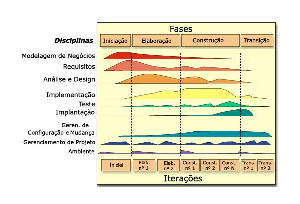
\includegraphics[scale=2.0]{figuras/abordagem/Fases_RUP}
    \caption{Gráfico RUP}
  \end{figure}

  As principais características do RUP são:

  \begin{itemize}
    \item \textbf{Casos de uso}: Tem como finalidade capturar os requisitos funcionais do sistema;
    \item \textbf{Centrado na arquitetura}: Base do projeto deve ser sólida e estável, mas podendo ser flexível para mudanças e incrementos, ou seja, o sistema deverá ser o mais modularizado possível;
    \item \textbf{Focado no risco}: Controla os riscos mais críticos logo no início da fase de Elaboração;
    \item \textbf{Baseado em componentes}: Artefatos são construídos a partir da interconexão de objetos projetados através da linguagem UML
  \end{itemize}

\section{Justificativa}

  A metodologia escolhida para este projeto foi o SAFe. Dentro dos fatores que levaram a essa escolha estão:

  \begin{itemize}
    \item A empresa é bastante nova, devido a isso, não sabem exatamente o que eles querem, levando a possíveis mudanças do escopo ao
          longo do projeto;
    \item Alguns dos integrantes da empresa já possuem experiência com o scrum;
    \item A presidente da empresa afirmou que poderia entrar em contato rapidamente com a nossa equipe caso houvesse algum problema;
    \item O diretor de recursos humanos da empresa é parente de um dos membros da equipe, facilitando ainda mais o contato com a empresa;
    \item Todos da equipe de desenvolvimento ja possuem experiência com a metodologia ágil.
    \item A equipe de desenvolvimento é pequena, podendo se auto gerenciar, uma das pregações do pensamento ágil;
  \end{itemize}

  De acordo com o Standish Group\cite{standishgroup}, a principal causa para o sucesso de um projeto é o envolvimento do cliente, e no
  nosso contexto, podemos facilmente obter esse envolvimento utilizando essa metodologia.

  \section{Maturidade}

  \subsection{CMMI (Capability Maturity Model $-$ Integration)}

    O CMMI é um modelo de maturidade internacional, geralmente utilizado por empresas
    globalizadas que necessitam de certificação para serem reconhecidos internacionalmente.
    Surgiu como integração e evolução dos modelos SW-CMM (Capability Maturity Model for Software),
    SECM EIA 731 (System Engineering Capability Model) e  e IPD-CMM
    (Integrated Product Development CMM).\cite{mct2006}.

    O CMMI possui 5 níveis de maturidade, enumerdos do 1 ao 5 e cada nível corresponde
    à capacidade da organização de desenvolvimento do produto, sendo o nível 1 o mais
    baixo nível de maturidade e o nível 5 o mais alto e contínuo.

    \begin{figure}[!ht]
      \centering
      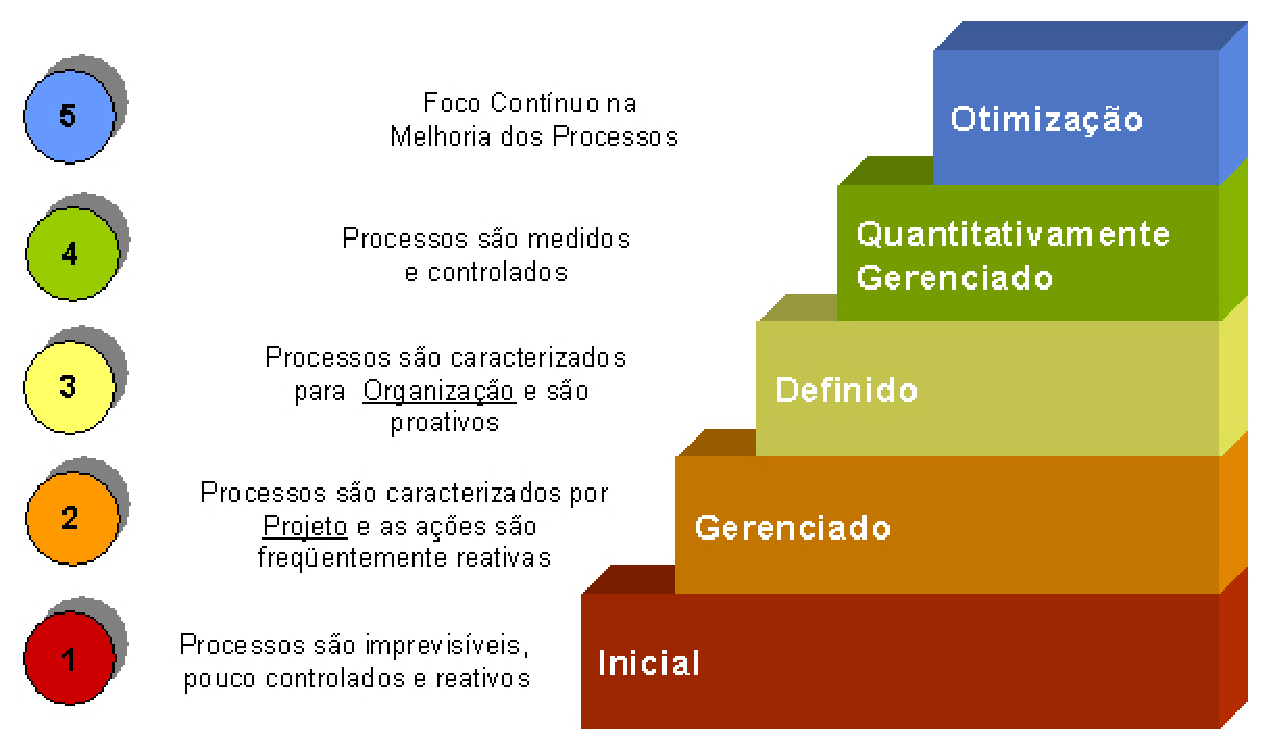
\includegraphics[width=15cm, keepaspectratio=true]{figuras/maturidade/niveis-cmmi.eps}
      \caption{Os cinco níveis de maturidade do modelo CMMI}
    \end{figure}

  \subsubsection{Vantagens}

    Como já dito na descrição na Subseção 1.1, o CMMI é um modelo de melhoria
    de processos reconhecido internacionalmente, fazendo com que a organização
    certificada por ele tenha a vantagem de ser reconhecida em qualquer lugar
    do mundo por causa da aplicação do CMMI

    Com o CMMI, a organização vai se otimizando cada vez mais e o controle do
    processo fica cada vez mais definido, sendo assim, a organização continuamente
    vai identificando o que realmente tem valor de acordo com sua maturidade.

  \subsubsection{Desvantagens}

    O CMMI tem um alto custo, por isso geralmente quem tem a certificação são
    grandes organizações globalizadas que possuem recursos para sustentar a
    avaliação e se torna vantajoso para seu reconhecimento internacional. O
    tempo para amadurecimento do processo pode levar de 4 a 8 anos, sendo assim
    definido um modelo moroso e caro. Segundo Franciscani, algumas organizações
    tratam o CMMi como um processo e não como modelo, fazendo com que eles tenham
    a percepção de que nem tudo que está no CMMI seja mesmo necesário.\cite{francis2012}.

  \subsection{MPS.BR}

    O modelo MPS.BR foi desenvolvido pela Softex com o objetivo de atingir
    certificações de pequenas e médias empresas, bem como possibilitar que
    as empresas possam ter acesso mais facilitado para a certificação.
    O modelo MPS.BR se adequa ao mercado brasileiro de software e deriva do CMMI
    Enquanto o CMMI possui cinco níveis de maturidade enumeradas do 1 ao 5, o
    MPS.BR possui sete níveis classificados, de forma piramidal,  pelas letras
    do A ao G, sendo o nível A o mais alto e contínuo nível de maturidade e o G
    o mais baixo. A Figura 2 contém a representação dos níveis de maturidade do
    MPS.BR

    \begin{figure}[!ht]
      \centering
      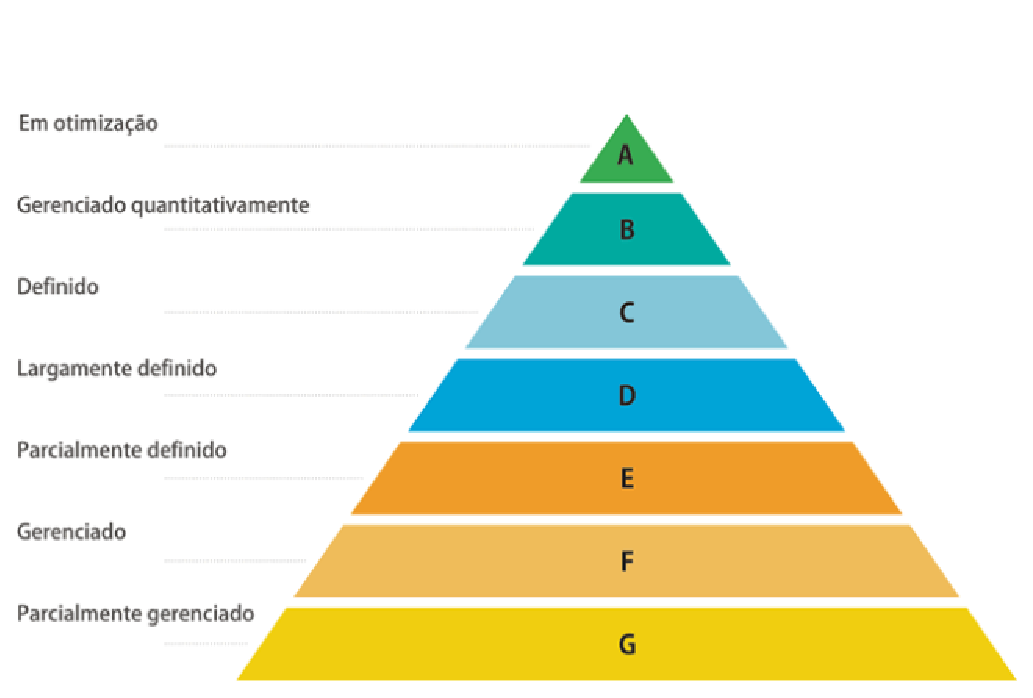
\includegraphics[width=15cm, keepaspectratio=true]{figuras/maturidade/niveis-mpsbr.eps}
      \caption{Os sete níveis de maturidade do modelo MPS.Br}
    \end{figure}

  \subsubsection{Vantagens}

    Além do MPS.BR ser mais acessível e estar mais adequado ao contexto de
    organizações brasileiras, segundo Franciscani, existem outras vantagens
    como:

    \begin{itemize}
      \item{Compatibilidade com CMMI, podendo ser aproveitado para uma futura
            certificação nesse modelo.}
      \item{Dois números de nível a mais do que do CMMI, o que pode facilitar a
            implantação em pequenas e médias organizações.}
      \item{Obrigatoriedade do certificado em licitações.}
      \item{Integração Universidade-Empresa.}
    \end{itemize}

  \subsubsection{Desvantagens}

    O MPS.BR não possibilita as empresas serem competitivas internacionalmente,
    por ser um modelo que se adequa apenas para certificação nacional. Isso pode
    ser uma desvantagem muito grande para organizações que pretendem
    globalizar-se.\cite{francis2012}.

  \subsection{Seleção do Modelo}

    A Cráton é uma empresa júnior com apenas 15 membros formada por estudantes no qual
    não visam lucro para si mesmos, pois todo o dinheiro obtido deve ser investido
    na própria empresa como consta na lei número 13.267 de 2016 que regulamenta as empresas
    juniores e as define com fim educacional e não lucrativo. Neste contexto, o CMMI seria
    impraticável devido ao alto custo e a limitação de crescimento de uma empresa júnior que é
    completamente dependente das universidades e não seria globalizada, não precisando do CMMI

    O grupo possui quatro integrantes, o que se encaixa no contexto do MPS.BR que se direciona
    principalmente para organizações menores, fazendo-se ser mais acessível para poder desenvolver
    o modelo dentro do contexto do cliente.

    O cliente, sendo uma empresa júnior integrada com a Universidade de Brasília, poderia se
    beneficiar dos processos do MPS.BR, já que é um modelo que possui integração universidade-empresa.
    Dessa forma, o modelo seria aplicado diretamente no meio acadêmico.

    Por esses motivos apontados, o modelo MPS.BR foi selecionado para a engenharia de requisitos da
    solução do problema da Cráton.

  \subsection{Processos Selecionados}

    Para o contexto da disciplina, serão implementados dois processos que tratam de
    requisitos, sendo o processo de Gerência de Requisitos que se encontra no nível
    G do MPS.BR e o Desenvolvimento de Requisitos que é um processo do nível D. Nos
    subtópicos seguintes, 1.4.1 e 1.4.2, estará o propósito e os resultados esperados
    de cada processo referenciado diretamente do Guia Geral do MPS.BR.\cite{softexmps}.

  \subsubsection{Gerência de Requisitos $-$ GRE}

    \begin{description}
      \item[Propósito] \
        O propósito do processo Gerência de Requisitos é gerenciar os requisitos do
        produto e dos componentes do produto do projeto e identificar inconsistências
        entre os requisitos, os planos do projeto e os produtos de trabalho do projeto.
      \item [Resultados Esperados] \
        \begin{itemize}
          \item GRE 1. O entendimento dos requisitos é obtido junto aos fornecedores de requisitos;
          \item GRE 2. Os requisitos são avaliados com base em critérios objetivos e um comprometimento
                da equipe técnica com estes requisitos é obtido;
          \item GRE 3. A rastreabilidade bidirecional entre os requisitos e os produtos de trabalho
                é estabelecida e mantida;
          \item GRE 4. Revisões em planos e produtos de trabalho do projeto são realizadas;
                visando identificar e corrigir inconsistências em relação aos requisitos;
          \item GRE 5. Mudanças nos requisitos são gerenciadas ao longo do projeto.
        \end{itemize}
      \end{description}

  \subsubsection{Desenvolvimento de Requisitos $-$ DRE}

    \begin{description}
      \item [Propósito] \
       O propósito do processo Desenvolvimento de Requisitos é definir os requisitos
       do cliente, do produto e dos componentes do produto.
      \item [Resultados Esperados]\
        \begin{itemize}
          \item DRE 1. As necessidades, expectativas e restrições do cliente, tanto do produto
                quanto de suas interfaces, são identificadas;
          \item DRE 2. Um conjunto definido de requisitos do cliente é especificado e priorizado
                a partir das necessidades, expectativas e restrições identificadas;
          \item DRE 3. Um conjunto de requisitos funcionais e não-funcionais, do produto e dos componentes
                      do produto que descrevem a solução do problema a ser resolvido, é definido e mantido
                      a partir dos requisitos do cliente;
          \item DRE 4. Os requisitos funcionais e não-funcionais de cada componente do produto são
                refinados, elaborados e alocados;
          \item DRE 5. Interfaces internas e externas do produto e de cada componente do produto são
                definidas;
          \item DRE 6. Conceitos operacionais e cenários são desenvolvidos;
          \item DRE 7. Os requisitos são analisados, usando critérios definidos, para balancear
                as necessidades dos interessados com as restrições existentes;
          \item DRE 8. Os requisitos são validados.
        \end{itemize}
    \end{description}
